\begin{figure}[htbp]
\centering
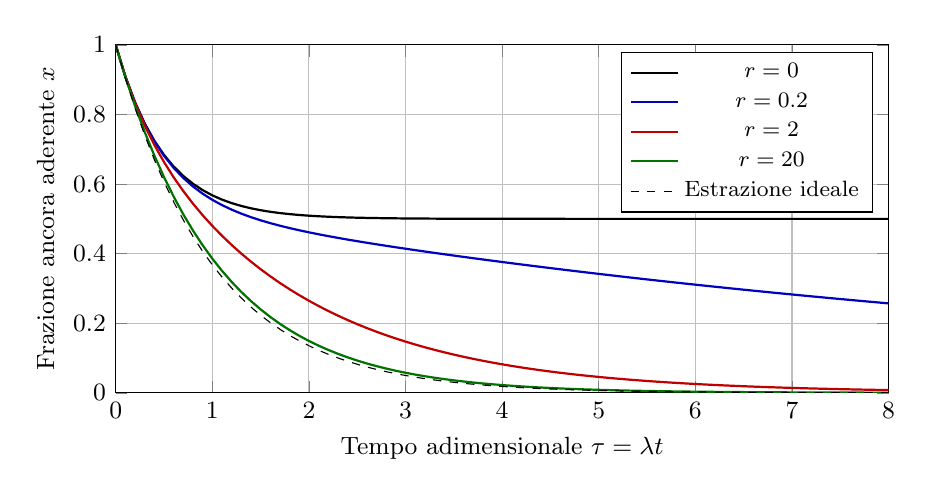
\begin{tikzpicture}
\begin{axis}[width=0.94\textwidth,height=6.0cm,xlabel={Tempo adimensionale $\tau=\lambda t$},ylabel={Frazione ancora aderente $x$},xmin=0,xmax=8,ymin=0,ymax=1,grid=major,legend style={font=\footnotesize,at={(0.98,0.98)},anchor=north east},tick label style={font=\small},label style={font=\small}]
\addplot[thick,black] coordinates {(0,1) (0.1,0.9093654) (0.2,0.83516) (0.3,0.7744058) (0.4,0.7246645) (0.5,0.6839397) (0.6,0.6505971) (0.7,0.6232985) (0.8,0.6009483) (0.9,0.5826494) (1,0.5676676) (1.1,0.5554016) (1.2,0.545359) (1.3,0.5371368) (1.4,0.530405) (1.5,0.5248935) (1.6,0.5203811) (1.7,0.5166866) (1.8,0.5136619) (1.9,0.5111854) (2,0.5091578) (2.1,0.5074978) (2.2,0.5061387) (2.3,0.5050259) (2.4,0.5041149) (2.5,0.503369) (2.6,0.5027583) (2.7,0.5022583) (2.8,0.5018489) (2.9,0.5015138) (3,0.5012394) (3.1,0.5010147) (3.2,0.5008308) (3.3,0.5006802) (3.4,0.5005569) (3.5,0.5004559) (3.6,0.5003733) (3.7,0.5003056) (3.8,0.5002502) (3.9,0.5002049) (4,0.5001677) (4.1,0.5001373) (4.2,0.5001124) (4.3,0.5000921) (4.4,0.5000754) (4.5,0.5000617) (4.6,0.5000505) (4.7,0.5000414) (4.8,0.5000339) (4.9,0.5000277) (5,0.5000227) (5.1,0.5000186) (5.2,0.5000152) (5.3,0.5000125) (5.4,0.5000102) (5.5,0.5000084) (5.6,0.5000068) (5.7,0.5000056) (5.8,0.5000046) (5.9,0.5000038) (6,0.5000031) (6.1,0.5000025) (6.2,0.5000021) (6.3,0.5000017) (6.4,0.5000014) (6.5,0.5000011) (6.6,0.5000009) (6.7,0.5000008) (6.8,0.5000006) (6.9,0.5000005) (7,0.5000004) (7.1,0.5000003) (7.2,0.5000003) (7.3,0.5000002) (7.4,0.5000002) (7.5,0.5000002) (7.6,0.5000001) (7.7,0.5000001) (7.8,0.5000001) (7.9,0.5000001) (8,0.5000001)};
\addlegendentry{$r=0$}
\addplot[thick,blue!75!black] coordinates {(0,1) (0.1,0.9093353) (0.2,0.834943) (0.3,0.773743) (0.4,0.7232401) (0.5,0.6814123) (0.6,0.6466215) (0.7,0.6175407) (0.8,0.5930942) (0.9,0.5724109) (1,0.5547847) (1.1,0.5396435) (1.2,0.5265238) (1.3,0.5150498) (1.4,0.5049173) (1.5,0.4958794) (1.6,0.4877362) (1.7,0.4803257) (1.8,0.4735164) (1.9,0.4672019) (2,0.4612957) (2.1,0.4557279) (2.2,0.4504416) (2.3,0.4453907) (2.4,0.4405378) (2.5,0.4358525) (2.6,0.4313101) (2.7,0.4268906) (2.8,0.4225776) (2.9,0.4183577) (3,0.4142203) (3.1,0.4101564) (3.2,0.4061589) (3.3,0.4022217) (3.4,0.3983401) (3.5,0.39451) (3.6,0.3907281) (3.7,0.3869917) (3.8,0.3832986) (3.9,0.3796468) (4,0.3760346) (4.1,0.3724608) (4.2,0.3689243) (4.3,0.3654239) (4.4,0.3619588) (4.5,0.3585283) (4.6,0.3551317) (4.7,0.3517685) (4.8,0.348438) (4.9,0.3451397) (5,0.3418733) (5.1,0.3386383) (5.2,0.3354343) (5.3,0.3322609) (5.4,0.3291178) (5.5,0.3260046) (5.6,0.3229211) (5.7,0.3198668) (5.8,0.3168416) (5.9,0.3138451) (6,0.3108769) (6.1,0.3079369) (6.2,0.3050248) (6.3,0.3021402) (6.4,0.299283) (6.5,0.2964528) (6.6,0.2936493) (6.7,0.2908724) (6.8,0.2881218) (6.9,0.2853972) (7,0.2826984) (7.1,0.2800251) (7.2,0.2773771) (7.3,0.2747541) (7.4,0.272156) (7.5,0.2695824) (7.6,0.2670331) (7.7,0.264508) (7.8,0.2620067) (7.9,0.2595291) (8,0.2570749)};
\addlegendentry{$r=0.2$}
\addplot[thick,red!75!black] coordinates {(0,1) (0.1,0.909078) (0.2,0.8331708) (0.3,0.7685775) (0.4,0.7126311) (0.5,0.6634017) (0.6,0.6194848) (0.7,0.5798518) (0.8,0.5437427) (0.9,0.5105898) (1,0.4799642) (1.1,0.4515367) (1.2,0.4250503) (1.3,0.4003011) (1.4,0.3771236) (1.5,0.3553811) (1.6,0.3349583) (1.7,0.3157562) (1.8,0.2976884) (1.9,0.2806782) (2,0.2646569) (2.1,0.2495622) (2.2,0.2353369) (2.3,0.2219286) (2.4,0.2092886) (2.5,0.1973715) (2.6,0.1861352) (2.7,0.1755401) (2.8,0.1655492) (2.9,0.1561277) (3,0.147243) (3.1,0.1388643) (3.2,0.1309626) (3.3,0.1235107) (3.4,0.116483) (3.5,0.1098553) (3.6,0.1036048) (3.7,0.09770993) (3.8,0.09215052) (3.9,0.08690745) (4,0.08196271) (4.1,0.07729933) (4.2,0.07290128) (4.3,0.06875348) (4.4,0.06484167) (4.5,0.06115243) (4.6,0.0576731) (4.7,0.05439173) (4.8,0.05129706) (4.9,0.04837846) (5,0.04562592) (5.1,0.04302999) (5.2,0.04058176) (5.3,0.03827282) (5.4,0.03609525) (5.5,0.03404158) (5.6,0.03210475) (5.7,0.03027812) (5.8,0.02855542) (5.9,0.02693073) (6,0.02539848) (6.1,0.02395341) (6.2,0.02259056) (6.3,0.02130525) (6.4,0.02009307) (6.5,0.01894985) (6.6,0.01787168) (6.7,0.01685486) (6.8,0.01589589) (6.9,0.01499147) (7,0.01413852) (7.1,0.0133341) (7.2,0.01257544) (7.3,0.01185995) (7.4,0.01118517) (7.5,0.01054878) (7.6,0.009948593) (7.7,0.009382559) (7.8,0.008848729) (7.9,0.008345273) (8,0.007870461)};
\addlegendentry{$r=2$}
\addplot[thick,green!45!black] coordinates {(0,1) (0.1,0.9074075) (0.2,0.8249234) (0.3,0.7501247) (0.4,0.6821311) (0.5,0.6203034) (0.6,0.5640801) (0.7,0.5129527) (0.8,0.4664595) (0.9,0.4241804) (1,0.3857334) (1.1,0.3507711) (1.2,0.3189778) (1.3,0.2900662) (1.4,0.2637751) (1.5,0.2398669) (1.6,0.2181258) (1.7,0.1983552) (1.8,0.1803766) (1.9,0.1640276) (2,0.1491604) (2.1,0.1356407) (2.2,0.1233465) (2.3,0.1121665) (2.4,0.1019999) (2.5,0.09275484) (2.6,0.08434769) (2.7,0.07670255) (2.8,0.06975036) (2.9,0.0634283) (3,0.05767926) (3.1,0.05245131) (3.2,0.0476972) (3.3,0.04337401) (3.4,0.03944266) (3.5,0.03586764) (3.6,0.03261665) (3.7,0.02966033) (3.8,0.02697197) (3.9,0.02452727) (4,0.02230416) (4.1,0.02028255) (4.2,0.01844417) (4.3,0.01677242) (4.4,0.0152522) (4.5,0.01386976) (4.6,0.01261263) (4.7,0.01146944) (4.8,0.01042987) (4.9,0.009484523) (5,0.008624861) (5.1,0.007843118) (5.2,0.007132231) (5.3,0.006485777) (5.4,0.005897916) (5.5,0.005363339) (5.6,0.004877215) (5.7,0.004435152) (5.8,0.004033157) (5.9,0.003667598) (6,0.003335173) (6.1,0.003032878) (6.2,0.002757983) (6.3,0.002508004) (6.4,0.002280683) (6.5,0.002073965) (6.6,0.001885984) (6.7,0.001715042) (6.8,0.001559593) (6.9,0.001418234) (7,0.001289688) (7.1,0.001172793) (7.2,0.001066493) (7.3,0.0009698274) (7.4,0.0008819238) (7.5,0.0008019877) (7.6,0.0007292968) (7.7,0.0006631945) (7.8,0.0006030837) (7.9,0.0005484211) (8,0.0004987131)};
\addlegendentry{$r=20$}
\addplot[black,dashed,domain=0:8,samples=80]{exp(-x)};
\addlegendentry{Estrazione ideale}
\end{axis}
\end{tikzpicture}
\caption{Modello di trasporto: $\beta=1$, con diversi ricambi $r$. Parametri scelti, non stimati sul campione. Il ricambio riduce il riadsorbimento ma non supera la velocit\`a intrinseca di distacco.}
\label{fig:transport}
\end{figure}
\begin{figure}[htbp]
\centering
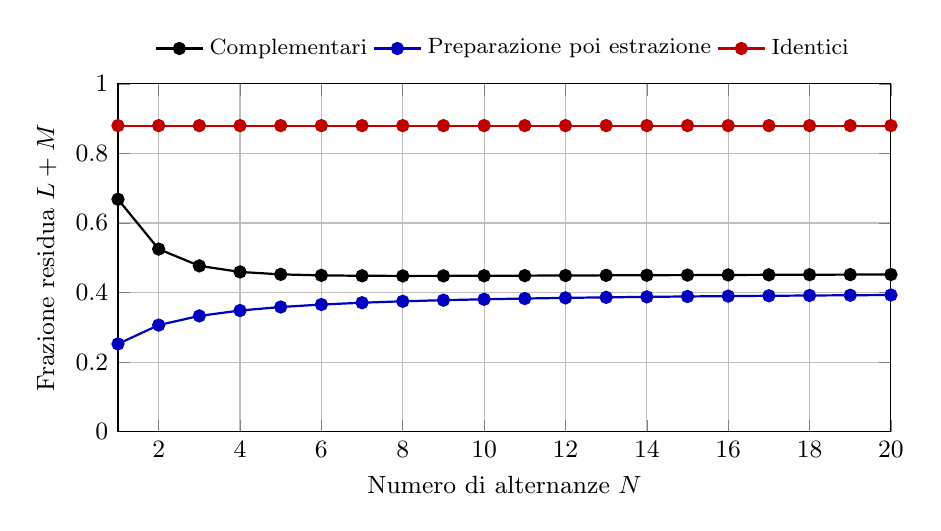
\begin{tikzpicture}
\begin{axis}[width=0.94\textwidth,height=6.0cm,xlabel={Numero di alternanze $N$},ylabel={Frazione residua $L+M$},xmin=1,xmax=20,ymin=0,ymax=1,grid=major,legend columns=3,legend style={font=\footnotesize,at={(0.5,1.04)},anchor=south,draw=none},tick label style={font=\small},label style={font=\small}]
\addplot[thick,black,mark=*] coordinates {(1,0.6680496) (2,0.5248837) (3,0.4766819) (4,0.4592498) (5,0.452253) (6,0.4493265) (7,0.4481709) (8,0.4478442) (9,0.4479215) (10,0.4481971) (11,0.4485664) (12,0.4489743) (13,0.4493913) (14,0.4498015) (15,0.4501966) (16,0.4505728) (17,0.4509283) (18,0.451263) (19,0.4515773) (20,0.4518724)};
\addlegendentry{Complementari}
\addplot[thick,blue!75!black,mark=*] coordinates {(1,0.2523549) (2,0.3064317) (3,0.3328908) (4,0.3483364) (5,0.3584219) (6,0.3655152) (7,0.3707725) (8,0.3748238) (9,0.3780406) (10,0.3806565) (11,0.3828253) (12,0.3846526) (13,0.3862129) (14,0.3875609) (15,0.3887371) (16,0.3897723) (17,0.3906905) (18,0.3915104) (19,0.392247) (20,0.3929124)};
\addlegendentry{Preparazione poi estrazione}
\addplot[thick,red!75!black,mark=*] coordinates {(1,0.8798123) (2,0.8798123) (3,0.8798123) (4,0.8798123) (5,0.8798123) (6,0.8798123) (7,0.8798123) (8,0.8798123) (9,0.8798123) (10,0.8798123) (11,0.8798123) (12,0.8798123) (13,0.8798123) (14,0.8798123) (15,0.8798123) (16,0.8798123) (17,0.8798123) (18,0.8798123) (19,0.8798123) (20,0.8798123)};
\addlegendentry{Identici}
\end{axis}
\end{tikzpicture}
\caption{Modello a stati conformazionali. Ogni curva mantiene invariati il tempo totale nel liquido D e quello nel liquido T. Alternare pi\`u spesso pu\`o aiutare o peggiorare: dipende dai tassi, qui illustrativi. D e T sono stati di trattamento ipotetici, non misure di DMF e THF.}
\label{fig:cycles}
\end{figure}
